%%%%%%%%%%%%%%%%%%%%%%%%%%%%%%%%%%%%%%%%%%%%%%%%%%%%%%%%%%%%%%%%%
%%% COSYNE-2007 Abstract Template
%%% Version 1.0
%%%%%%%%%%%%%%%%%%%%%%%%%%%%%%%%%%%%%%%%%%%%%%%%%%%%%%%%%%%%%%%%%

\documentclass[12pt,draft]{article}
\usepackage{times}
%\inner 0.5in
\oddsidemargin -0.5in		% margin, in addition to 1" standard
\textwidth 7.5in		% 8.5" - 2*(1+\oddsidemargin)

\topmargin -1in		% in addition to 1.5" standard margin
\textheight 9.75in 		% 11 - ( 1.5 + \topmargin + <bottom-margin> )

\columnsep 0.25in

\parindent 0pt
\parskip 12pt

\flushbottom \sloppy
\pagestyle{empty} % No page numbers

\usepackage{subfigure}
\usepackage{tikz}
\usepackage[sorting=none]{biblatex}
\usepackage{csquotes}
%\usepackage[footnotesize]{caption}


\bibliography{biblio}
%%%%%%%%%%% BEGIN METADATA %%%%%%%%%%%%
\newcommand{\AuthorAG}{Antoine Grimaldi}

\newcommand{\AuthorLP}{Laurent Perrinet}
\newcommand{\AuthorVB}{Victor Boutin}
\newcommand{\AddressLP}{Institut de Neurosciences de la Timone (UMR 7289); Aix Marseille Univ, CNRS; Marseille, France}%
\newcommand{\WebsiteLP}{https://laurentperrinet.github.io}%
\newcommand{\EmailLP}{Laurent.Perrinet@univ-amu.fr}%
\newcommand{\EmailRB}{xxx@xxx}%
\newcommand{\AuthorSI}{Sio-Hoi Ieng}
\newcommand{\AuthorRB}{Ryad Benosman}%
\newcommand{\orcidRB}{0000-0003-0243-944X}%
\newcommand{\AddressRB}{Sorbonne Université, INSERM, CNRS, Institut de la Vision, France;}%
\newcommand{\Abstract}{
A single paragraph of about 200 words maximum. For research articles, abstracts should give a pertinent overview of the work. We strongly encourage authors to use the following style of structured abstracts, but without headings: (1) Background: Place the question addressed in a broad context and highlight the purpose of the study; (2) Methods: Describe briefly the main methods or treatments applied; (3) Results: Summarize the article's main findings; and (4) Conclusion: Indicate the main conclusions or interpretations. The abstract should be an objective representation of the article, it must not contain results which are not presented and substantiated in the main text and should not exaggerate the main conclusions.
}

\begin{document}

%%%-----------------------------------------------------------------
{\Large\bf
Image classification using SNN
}

{\bf
\AuthorAG\ , \AuthorVB\ , \AuthorLP\ ,\AuthorSI\ and \AuthorRB}

{
Institut de Neurosciences de la Timone, Aix Marseille Univ / CNRS, Marseille, France.
}

%%%-----------------------------------------------------------------
%%SUMMARY

\parindent 12pt

\textbf{Summary}.

Reverse engineering is the art of looking at an existing device in order to understand its concepts and operation. We used this approach to link innovative methods used in computer vision to computational neuroscience. In Lagorce 2017 novel event-based spatio-temporal features are introduced: time-surfaces. Built from asynchronous events acquired by a neuromorphic camera time-surfaces allowed to use dynamics of a visual scene and to create an efficient hierarchical event-based pattern recognition architecture. This work is three-fold, first through the analysis of this existing method we were able to adapt its formalism in the computational neuroscience framework with a simple leaky integrate-and-fire neuron model and Hebbian learning. Then, after reproduction of their results, generalization of the classification task with a more complex and widely used dataset (N-MNIST) was performed using logistic regression. A significant contribution was to achieve online classification of the N-MNIST dataset reaching state of the art performances. To our knowledge it is the first end-to-end event-based online classification network. The third contribution came by adding an homeostatic regulation rule for neuron activity. According to the efficient coding hypothesis, neural activity should be equally distributed between neurons. We used this principle to force neurons in the same layer to spike with an equivalent probability by adding a gain depending on their past activity. Efficiency of this technique was demonstrated through an improvement in learning spatio-temporal patterns during the training phase and an improvement in classification performance reaching 97,8\% accuracy. By using methods used in a different field we were able to develop an efficient model for online digit classification. We aim at pursuing the study of this architecture through natural scene unsupervised learning and hope to get hints about efficient neural coding.

%%END OF SUMMARY



\begin{figure}[!ht]%[!ht][!b]%
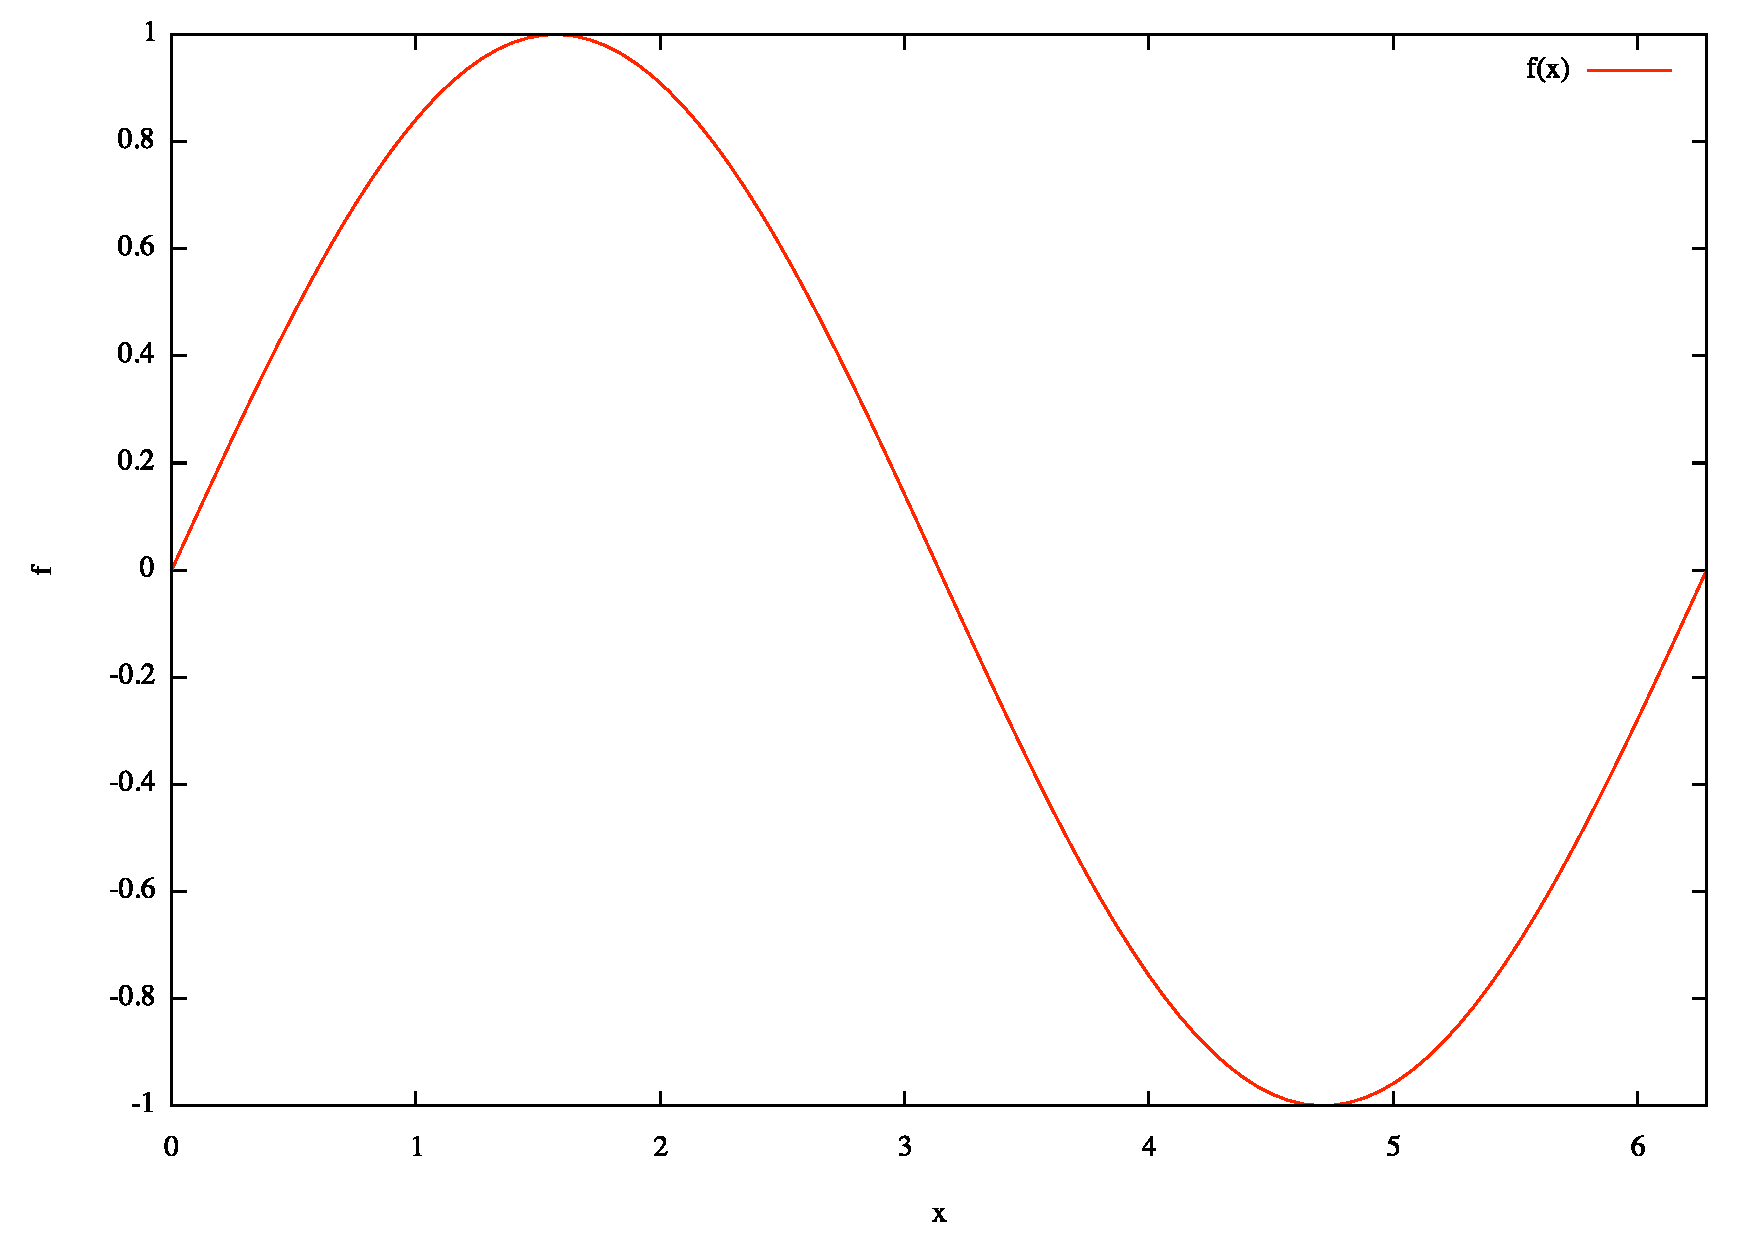
\includegraphics[width=0.99\linewidth]{figure1}
\end{figure}

\caption
{
\textbf{Figure 1}: (a)
%\label{fig:fig1}
}


\vfil

%%%-----------------------------------------------------------------
%{\bf Acknowledgments}\\
%We thank T. Colleague for helpful discussions.
%This work was supported by NIH grant DC999999.

%%%-----------------------------------------------------------------
\printbibliography

\end{document}
